\documentclass[unicode]{beamer}

\mode<presentation>
{
	\usetheme{Warsaw}
%	\setbeamertemplate{headline}{}
%	\setbeamertemplate{footline}{}
}

\usepackage[utf8]{inputenc}
\usepackage[T2A]{fontenc}
\usepackage{amssymb, amsmath, hyperref}
\usepackage[main=russian,english]{babel}

\title{Автоматическая транскрипция музыки (AMT)}
\author{Сергей Синяк}
\date{Минск, 2017}

\begin{document}

\begin{frame}
	\titlepage
\end{frame}

\section{Характеристика работы}
\begin{frame}
  За время работы над дипломом были рассмотрены различные подходы
  для решения задачи автоматической транскрипции музыки.
  Они включают преобразование фурье, константное Q преобразование,
  NMF и машинное обучение.
  Стоит отметить относительный успех применения нейронных сетей
  на базе датасета MAPS. Ведь только здесь удалось вернуться
  к исходной постановке задачи, а именно когда
  дан набор шаблонов наигранных нот и требуется распознать
  произвольную нотную последовательность исполненную на том же
  инструменте.
\end{frame}

\section{Содержание}

\begin{frame}
   Отметим план/содержание работы в экспериментах с нейронными сетями
  \begin{enumerate}
    \item Подготовка датасета
    \item Обработка данных и формирование тренировочной и тестовой выборок.
    \item Определение функции потерь и целевой функции точности.
    \item Эксперименты с архитектурой нейронной сети, её обучение и
      валидация
    \item Визуализация результата работы
  \end{enumerate}
\end{frame}

\section{Положения к защите}
\begin{frame}
\begin{figure}
  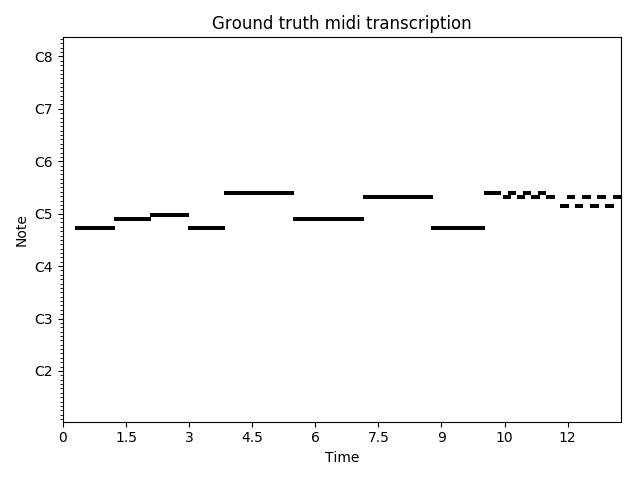
\includegraphics[scale=.6]{res/organ-note-groundtruth.png}
\end{figure}
\end{frame}

\begin{frame}
\begin{figure}
  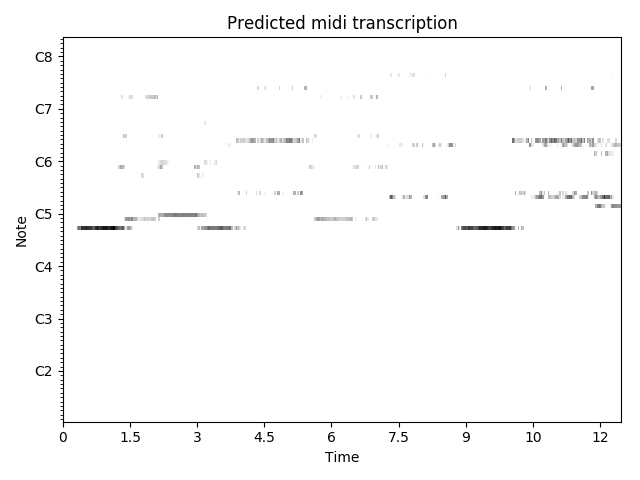
\includegraphics[scale=.6]{res/organ-overfit-028-acoustic.png}
\end{figure}
\end{frame}

\begin{frame}
\begin{figure}
    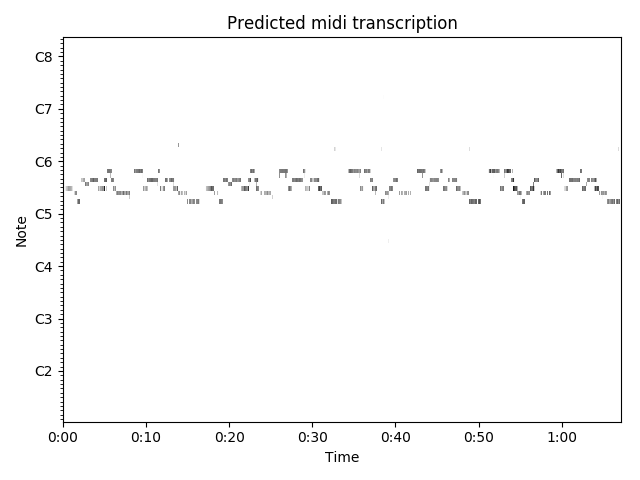
\includegraphics[scale=.64]
      {res/daj-ci-boze-dobranoc-overfit-028-acoustic.png}
\end{figure}
\end{frame}

\section{Заключение}

\begin{frame}
  \center{Спасибо за внимание!}
\end{frame}

\end{document}
